\chapter{Utilisation de Git}
Présentation réalisée par Pierre CHEVALIER.
\section{Résumé}
Git est un logiciel de gestion de versions décentralisé et libre développé notamment par Linus Torvalds et Junio Hamano. Il nous a permis de gérer les versions du projet conjointement avec le service d’hébergement de fichiers en ligne Github. Nous aurions également pu utiliser Git Server pour héberger nous-même les fichiers. Comme ce serveur aurait dû être lancé 24h/24 (car nous travaillions 24h/24) nous avons préféré utiliser une plateforme d’hébergement moins contraignante.

\noindent Les avantages notables de Git sont:
\begin{itemize}
	\item Chaque objet enregistré possède un identifiant universel en SHA1 qui permet de l’identifier de manière unique,
	\item Git est multi-protocole, ce qui signifie que les échanges peuvent se faire en ssh, http(s) etc,
	\item Les objets stockés sont compressés,
	\item Pas de relation client/serveur,
	\item Gestion efficaces des branches de développement.
\end{itemize}

Il peut être utilisé directement depuis un terminal, ce que nous faisions lorsque nous travaillions sur les terminaux de l’ISIMA, mais peut aussi être utilisé par d’autre logiciel  sous forme de plugin ou de programme dédié. Lors de développement du projet, nous avons notamment utilisé le logiciel de Github, Github Desktop, très utile dans le cadre d’une utilisation de Git sous Windows et non sous Linux ainsi que sous la forme d’un plugin intégré à Visual Studio.

Ces logiciels et plugin permettent une utilisation plus intuitive de Git, améliorant la vitesse de certaines actions prise par l’utilisateur.
\newpage
\noindent Quelques mots de vocabulaire:

\noindent
\begin{tabular}{p{0.1\textwidth}p{.85\textwidth}}
	Version & 
	On appelle version l’état du projet actuel, les fichiers présents, leur contenu etc. Git est un logiciel qui conserve toutes les versions enregistrées. \\
	
	Repository &
	Le répertoire. Dans ce rapport nous appellerons repository le répertoire git composé de toutes les versions enregistrées du projet. Le repository local est l’arborescence de version présente sur le disque dur de l’utilisateur, le repository distant est l’arborescence présente sur le serveur git. Lors d’un push ou d’un pull (d’un envoie de version ou une récupération de la version distante), les deux repositories se synchronisent. \\

	Commit &
	C’est un objet git (voir plus bas). On commit nos fichiers après une modification pour les enregistrer localement puis on les push pour envoyer les modifications au serveur.\\

	Branche &
	Une branche est une version de l’arborescence du projet. C’est-à-dire une mutation du projet avec ces propres versions. Elle permet notamment d’éviter les conflits récurrents lorsque deux développeurs travaillent sur des fichiers communs. Cette pratique part du principe de préféré faire une grosse fusion de la branche à la fin du développement plutôt que de faire une multitude de petites fusions à chaque fois qu’un des développeurs poste sur le repository distant. \\
	
	Clone &
	Un utilisateur de git peut cloner un repository. Git va copier toute l’arborescence du projet sur le disque dur de l’utilisateur. Celui-ci pourra ensuite envoyer ses propres commits sur le serveur distant s’il en a la permission. L’utilisateur peut aussi créer un nouveau repository en ligne basé sur cet ancien repository qu’il vient de cloner. \\

	Index &
	L’index est la dernière modification enregistrée par git (le dernier commit). Quand il faut envoyer les commit au repository distant, git va d’abord vérifier que son index est à jour avant d’envoyer. \\
	
	Conflit &
	Lorsque deux utilisateurs travaillent sur un même fichier, qu’ils le commit en même temps, il arrive que ces modifications soient issues d’une même version et donc lors de la mise à jour de repository distant (ou local si l’utilisateur n’a pas récupérer la dernière version enregistrée par le serveur distant) l’utilisateur peut être confronté à un conflit de fichier. Pour le résoudre, l’utilisateur peut choisir de conserver sa version locale ou la version distante ou encore faire une fusion des deux fichiers (il choisit quelles lignes conserver)
\end{tabular}

\section{Procédure d’installation}

Pour installer git sous un terminal il suffit  d’utiliser la commande suivante dans un terminal:
\begin{minted}{bash}
$ apt-get install git
\end{minted}

Si vous êtes sous Fedora, il faut utiliser la commande:
\begin{minted}{bash}
$ yum install git
\end{minted}

\noindent Tentez alors de lancer la commande \texttt{\$ git} pour vous assurer de la bonne installation du logiciel.

Si vous voulez également utiliser le service de cloud de Github, vous devez vous inscrire sur le site.

Pour installer Github Desktop il faut télécharger l’installateur à l’adresse suivante. Suivez les instructions et installer le logiciel. Celui-ci vous permettra d’installer de surcroit git sur votre ordinateur sous Windows en plus du logiciel Github Desktop.

Pour installer le plugin git sous Visual Studio il faut télécharger le plugin puis l’installer. Celui-ci vous permettra d’installer de surcroit git sur votre ordinateur sous Windows.

\section{Présentation des fonctionnalités}

Les logiciels de gestion de versions utilisent une arborescence de fichier permettant de conserver toutes les versions des fichiers et de mutualiser le développement entre les différents utilisateurs. Les développeurs mettent ainsi en ligne leur avancement accompagné d’un commentaire et le code source est mis à jour en fonction de cet avancement. Seuls les fichiers modifiés seront mis à jour. Un des avantages de ces logiciels est donc qu’ils limitent les doublons de données dans un projet qui peut être lourd en espace disque. Un autre avantage de ces logiciels est qu’ils permettent de gérer les conflits de version lorsque deux développeurs mettent leur avancement en ligne en même temps: une interface permet au dernier utilisateur qui a envoyé son travail de choisir quelles lignes garder.

Git se divise en deux structures de données: la base d’objets et le cache de répertoire. La base d’objet se trouve sur le disque dur client et se met à jour sur le serveur à chaque émission de versions et permet d’accéder à toutes les versions du projet alors que le cache de répertoire est uniquement sur la machine de l’utilisateur.

\noindent La base d’objet se compose de quatre types d’objet:
\begin{itemize} 
	\item         L’objet blob (binary large objects) qui correspond à une version d’un fichier
	\item         L’objet tree qui contient des objets blob comme un répertoire le ferait
	\item         L’objet commit qui donne accès à une arborescence (à un tree racine et vers ses commit parents). Il possède également un message de log.
	\item         L’objet tag qui est un message lié à un objet commit
\end{itemize}

Les actions possibles de l’utilisateur permettent d’ajouter et de supprimer ces objets.

Ces objets sont stockés dans le répertoire caché .git (situé dans le cache de répertoire). Le répertoire .git contient également des fichiers de configuration de l’environnement git, des informations sur les branches locales du repository, des logs, des infos sur l’état du prochain commit ...

\subsection{Git dans le terminal}
Le logiciel Git sous terminal consiste en une multitude de commandes permettant de créer des répertoires git, de récupérer les mises à jour distantes et d’exporter les mises à jour locales. Voici la liste des commandes les plus utilisées durant le projet et leur explication.

\noindent Commandes les plus utilisées:
\begin{itemize}
\item \textbf{git init:} Permet d’initialiser un repository sur le disque dur. Il va ainsi créer le .git d’un nouveau projet.
\item \textbf{git clone:} Permet de créer une copie d’un repository existant en ligne. L’utilisateur a alors accès à ce repository et peut même faire des commit (si cette utilisateur est autorisé par le serveur)
\item \textbf{git add:} Ajoute des fichiers de l’index du repository courant
\item \textbf{git rm:} Supprime des fichiers de l’index du repository courant
\item \textbf{git commit:} Prends tout les changements de l’index et crée un nouvel objet commit et sauvegarde cet objet en local. Un commentaire doit être associé à cet objet. Cette commande met à jour l’index du repository .
\item \textbf{git status:} Montre les différences qu’il y a entre le répertoire réel et l’index de repository. Il va lister les fichiers non enregistrés dans l’index, les fichiers modifiés et les fichiers prêts à l’envoie (c’est-à-dire dont la version a été enregistrée dans un objet commit)
\item \textbf{git branch:} Liste les branches existantes sur le projet. Crée une nouvelle branche si un nom est donné en argument.
\item \textbf{git checkout:} Permet de changer de branche.
\item \textbf{git merge:} Permet de fusionner deux branches. Cette action va automatique créer un nouveau commit s’il n’y a pas de conflits. Dans l’autre cas l’utilisateur va être invité à opérer à une fusion de fichiers ou à conserver une version.
\item \textbf{git reset:} Permet de retourner à la version du dernier objet commit crée (version de l’index).
\item \textbf{git pull:} Permet de récupérer les fichiers sur le repository distance vers le repository local. Equivalent à git fetch
\item \textbf{git push:} Permet d’envoyer les objets commit locaux au repository distant.
\item \textbf{git log:} Montre la liste des commit de la branche courante et les détails correspondants (les tags et les lignes modifiées par exemple)
\item \textbf{git show:} Montre les détails des commits locaux
\end{itemize}
\noindent Autres commandes:
\begin{itemize}
\item \textbf{git config:} Permet de configure le nom, l’email, etc de l’utilisateur
\item \textbf{git stash:} Sauvegarde des modifications que l’on ne veut pas commit immédiatement. Les changements pourront être appliqués plus tard.
\item \textbf{git tag:} Lie un message (un objet Tag) à un commit.
\item \textbf{git fetch:} Permet de récupérer les fichiers sur le repository distant vers le repository local
\item \textbf{git remote:} Montre toutes les versions distantes du repository
\item \textbf{git ls-tree:} Montre l’objet tree en incluant le nom de chaque objets et leur valeur en SHA-1
\item \textbf{git cat-file:} Prend en argument la valeur en SHA-1 d’un objet et permet de voir un objet
\item \textbf{git grep:} permet de faire une recherche à partir d’un mot clef dans un objet tree
\item \textbf{git diff:} Affiche les différences entre les modifications de l’index et celle du répertoire courant
\end{itemize}
L’avantage de cette interface commande est qu’elle permet une grande marge de manœuvre à l’utilisateur puisque celui-ci à accès à l’ensemble des commandes git et donc à un contrôle total de son repository. L’inconvénient le manque d’intuitivité de certaine commande.

\subsection{Git avec Github Desktop}

Github Desktop est un logiciel fournit par Github mais qui peut également être utilisé sur des plateformes d’hébergement autres que Github puisque l’installation du logiciel donne aussi accès à une interface en ligne de commande de Git, donnant accès de ce fait à toutes les commandes Git. On peut ainsi cloner des repositories sur des serveurs externes à Github tout en profitant quand même de l’interface graphique.

\begin{center}
	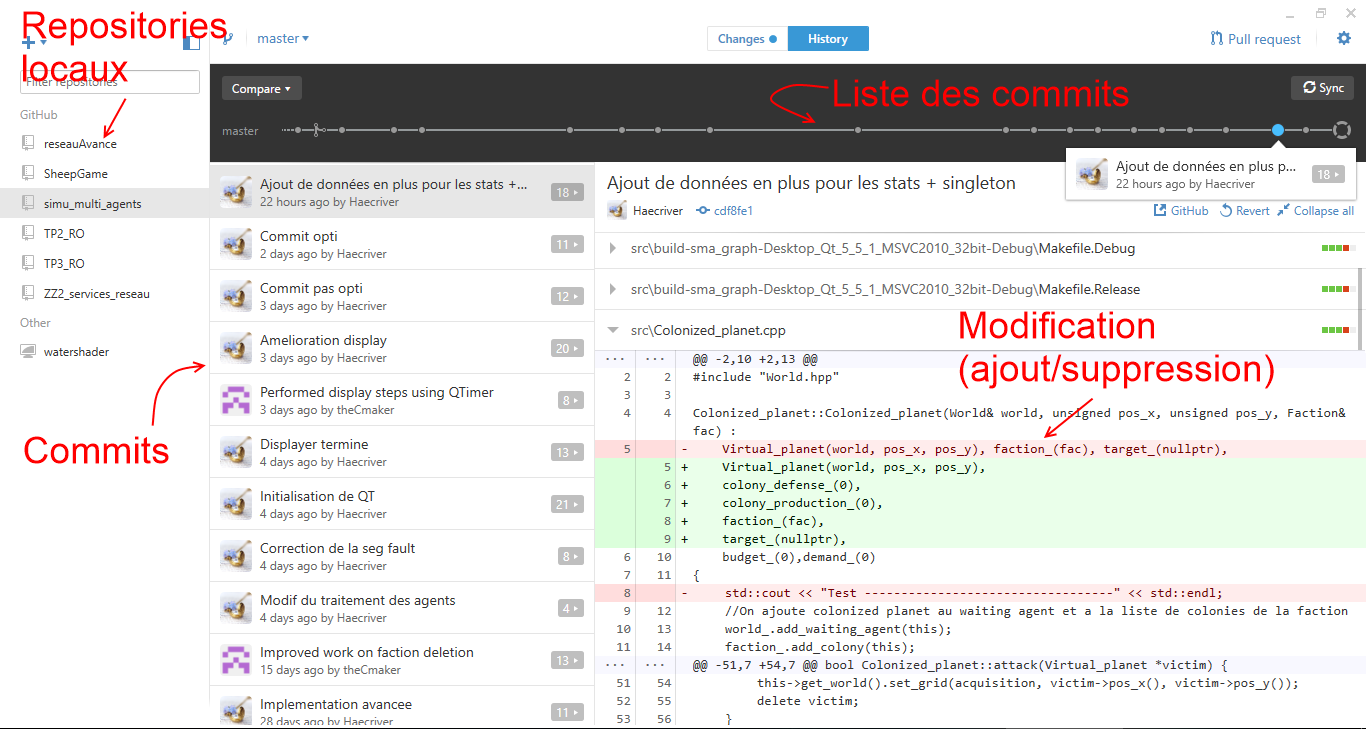
\includegraphics[width=\textwidth]{images/commit.png}
\end{center}
 
Celle-ci possède des capacités plus limité que l’interface commande. Par exemple on ne peut pas cloner un directement depuis l’interface graphique un  repository d’un serveur git distant (qui n’est pas Github) mais en contrepartie les merges sont plus intuitifs et la présentation des branches et commit est plus ergonomique.

\subsection{Git avec Visual Studio}

Le plugin de Visual Studio, tout comme le logiciel Github Desktop n’est pas aussi puissant que l’interface commande mais permet d’afficher l’historique des commits et surtout possède une interface facilitant grandement les merges si bien que nous n’avons pas eu besoin de travailler sur des branches durant le projet (sachant que celui-ci était réduit par rapport à de vrais projets professionnels bien entendu).

L’interface se présente ainsi:

\begin{center}
	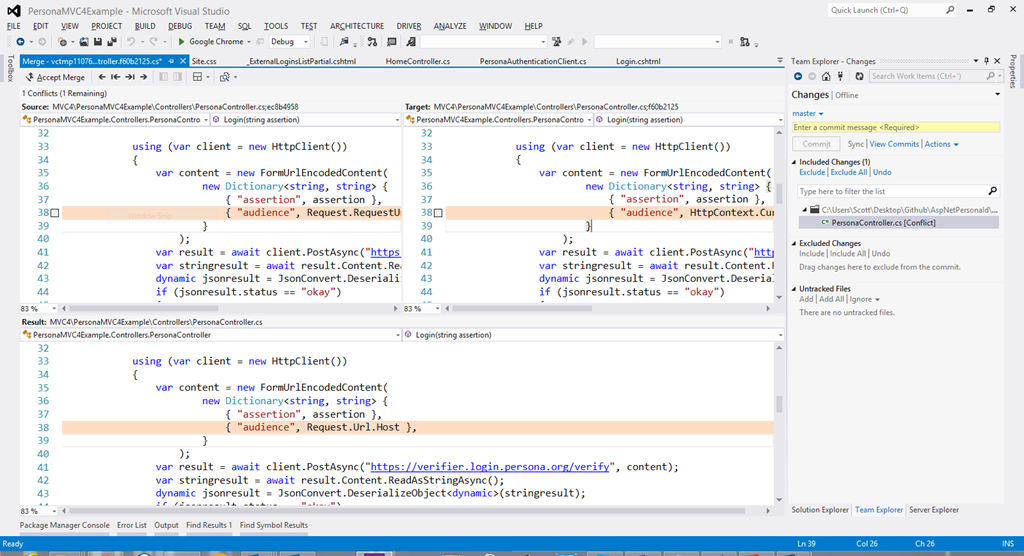
\includegraphics[width=.8\textwidth]{images/visual.png}
\end{center}

Visual présente les deux versions en conflit avec une case à cocher pour savoir quelle version conserver. Le résultat est affiché en dessous des deux fenêtres. Un bouton permet de passer rapidement au conflit suivant. S’il y a un problème ambigu, l’utilisateur peut toujours modifier le résultat à la main.
 
\noindent Références:\\
\href{https://git-scm.com/}{\texttt{https://git-scm.com/}}\\
\href{http://igm.univ-mlv.fr/~dr/XPOSE2008/git/fonctionnement.html}{\texttt{http://igm.univ-mlv.fr/~dr/XPOSE2008/git/fonctionnement.html}}\\
\href{https://www.siteground.com/tutorials/git/commands.htm}{\texttt{https://www.siteground.com/tutorials/git/commands.htm}}\\
\href{https://fr.wikipedia.org/wiki/Git}{\texttt{https://fr.wikipedia.org/wiki/Git}}\\
\href{https://fr.wikipedia.org/wiki/GitHub}{\texttt{https://fr.wikipedia.org/wiki/GitHub}}

\noindent Image merge visual:\\
\href{http://www.hanselman.com/blog/content/binary/Windows-Live-Writer/ed5b594103c4\_B6D0/image\_2.png}{\texttt{http://www.hanselman.com/blog/content/binary/Windows-Live-Writer/ed5b594103c4\_B6D0/image\_2.png}}